\documentclass[11pt,letterpaper]{article}
\usepackage[lmargin=1in,rmargin=1in,tmargin=1in,bmargin=1in]{geometry}
\usepackage{../style/homework}
\usepackage{../style/commands}
\setbool{quotetype}{false} % True: Side; False: Under
\setbool{hideans}{true} % Student: True; Instructor: False

% -------------------
% Content
% -------------------
\begin{document}

\homework{10: Due 04/27}{An approximate answer to the right problem is worth a good deal more than an exact answer to an approximate problem.}{John Tukey}

% Problem 1
\problem{10} Find the least square regression line, along with the $r$ and $r^2$ value, for the dataset $\{ (-1, -2), (1, 3), (2, 2), (4, 5) \}$. Show all your work. 



\newpage



% Problem 2
\problem{10} Given the following information below, find the least square regression line. Show all your work. 
	\[
	\begin{aligned}
	n&= 10 \\
	\overline{x}&= 19.59, \quad s_x^2&= 2.9225 \\
	\overline{y}&= 15.63, \quad s_y^2&= 5.2407 \\
	R&= 0.8733
	\end{aligned}
	\]



\newpage



% Problem 3
\problem{10} Match each regression coefficient to its corresponding graph. 
	\begin{figure}[!ht]
	\centering
	\begin{minipage}{0.45\textwidth}
	   \centering
	   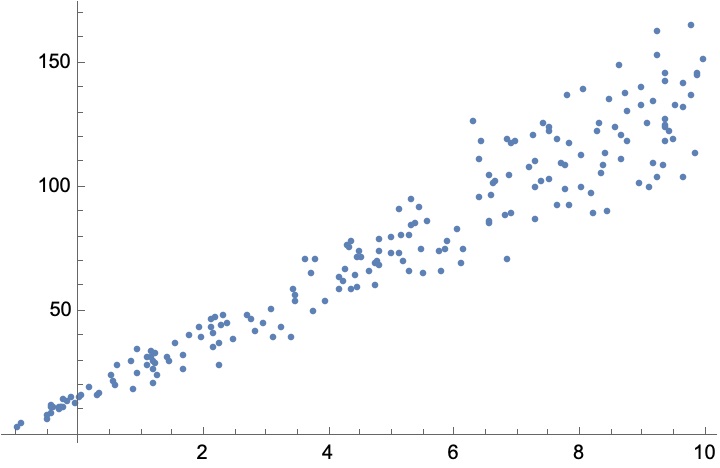
\includegraphics[width=0.9\textwidth]{reg1.png}
	   \caption*{(a)}
	\end{minipage}\hfill
	\begin{minipage}{0.45\textwidth}
	   \centering
	   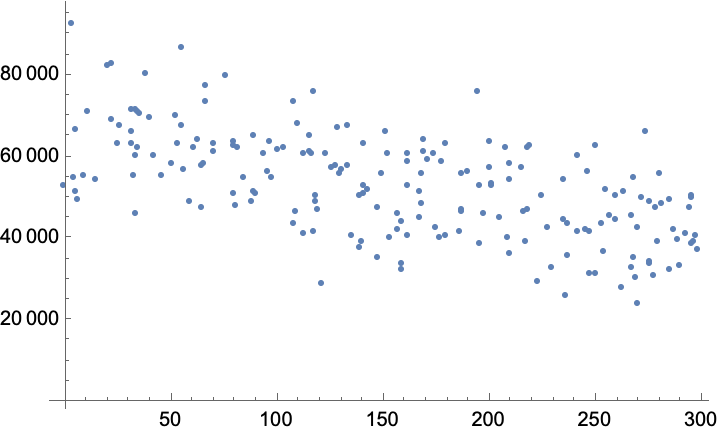
\includegraphics[width=0.9\textwidth]{reg2.png}
	   \caption*{(b)}
	\end{minipage}
	\begin{minipage}{0.45\textwidth}
	   \centering
	   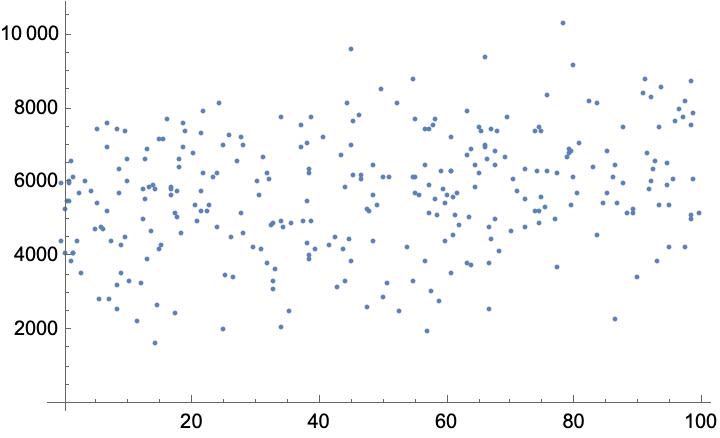
\includegraphics[width=0.9\textwidth]{reg3.png}
	   \caption*{(c)}
	\end{minipage}
	\begin{minipage}{0.45\textwidth}
	   \centering
	   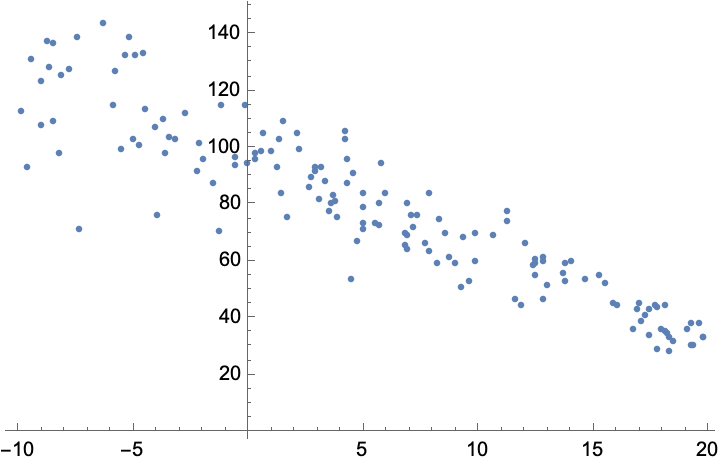
\includegraphics[width=0.9\textwidth]{reg4.png}
	   \caption*{(d)}
	\end{minipage}
	\end{figure}

\begin{enumerate}[(i)]
\item \underline{\hspace{1.5cm}}: $R= -0.9197$
\item \underline{\hspace{1.5cm}}: $R= -0.6023$
\item \underline{\hspace{1.5cm}}: $R= 0.2527$
\item\underline{\hspace{1.5cm}}: $R= 0.9616$
\end{enumerate} 



\newpage



% Problem 4
\problem{10} A researcher is trying to predict home run records. The researcher wants to predict what the next home run record will be. To model this, they will take the last ten home run records and label them as $r= 1, 2, \ldots, 10$, i.e. $r= 1$ is the tenth highest home run record, $r= 2$ is the ninth highest home run record, etc.. They fit a linear regression to this data and find a simple linear regression model of $h(r)= 20.21r + 559.3$. 
	\begin{enumerate}[(a)]
	\item What are $b_0$ and $b_1$ for this linear regression?
	\item Predict the future home run record by finding $h(11)$.
	\item For $r= 8$, the home run record, $h(8)$, was known to be Babe Ruth's record of 714 home runs. Find the residual for this value given the model.
	\item The researcher finds an $R^2$ value of $0.9837$. Is the linear model a good fit to the home run record data? Explain. 
	\end{enumerate}


\end{document}